%\documentclass[a4,semhelv,landscape]{seminar}
\documentclass[landscape]{slides}
%\documentclass[pdf, default, slideBW, nocolorBG]{prosper}
\usepackage[left=0.2cm,top=0.2cm,right=0.2cm,bottom=0.2cm,nohead,nofoot]{geometry}
%\def\everyslide{\sffamily}
%\usepackage{fullpage}
\usepackage{graphicx}
\usepackage[usenames]{color}
%\usepackage{color}
\usepackage{verbatim}
\usepackage{nopageno}
\usepackage{setspace}
%\usepackage{times}
% define some nice colors
\definecolor{myred}{rgb}{0.6,0,0}
\definecolor{myblue}{rgb}{0,0.2,0.4}
\definecolor{mygreen}{rgb}{0,0.5,0.0}
\definecolor{mypurple}{cmyk}{0.5,1.0,0.0,0.0}
\definecolor{myorange}{cmyk}{0.0,0.75,1.0,0.0}
%\color{myblue}

\begin{document}
%%%%%%%%%%%%%%%%%%%%%%%%%%%%%%%%%%%%%%%%%%%%%%%%%%%%%%%%%%%%%%%%%%%%%%
\begin{slide}
\begin{center}
\textbf{Rfam: RNA families database (3016 families)}

\small
\begin{itemize}
\item Each family is represented by:
  \begin{itemize}
  \item representative SEED alignment annotated with secondary-structure
  \item covariance model (CM) built from the SEED
  \item hits in Rfamseq database above GA threshold (FULL)
  \end{itemize}
\end{itemize}

\vspace{0.5in}
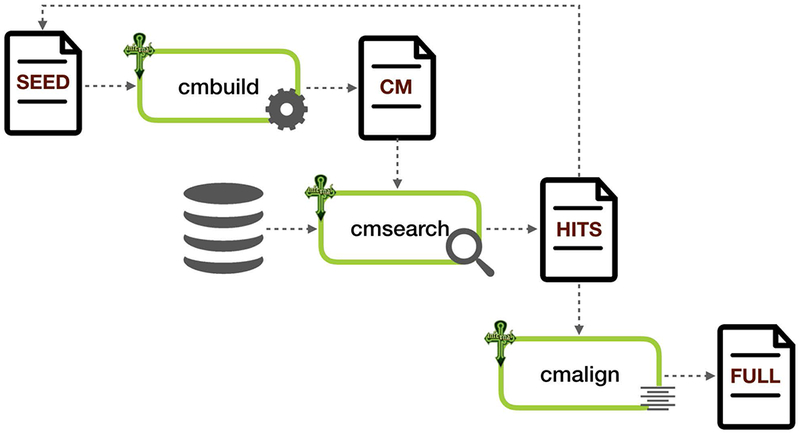
\includegraphics[height=5in]{figs/kalvari18-rfam-schema}

\vfill
\tiny \flushleft{Kalvari et al., 2018}
\end{center}
\end{slide}
%%%%%%%%%%%%%%%%%%%%%%%%%%%%%%%%%%%%%%%%%%%%%%%%%%%%%%%%%%%%%%%%%%%%
\begin{slide}
\begin{center}
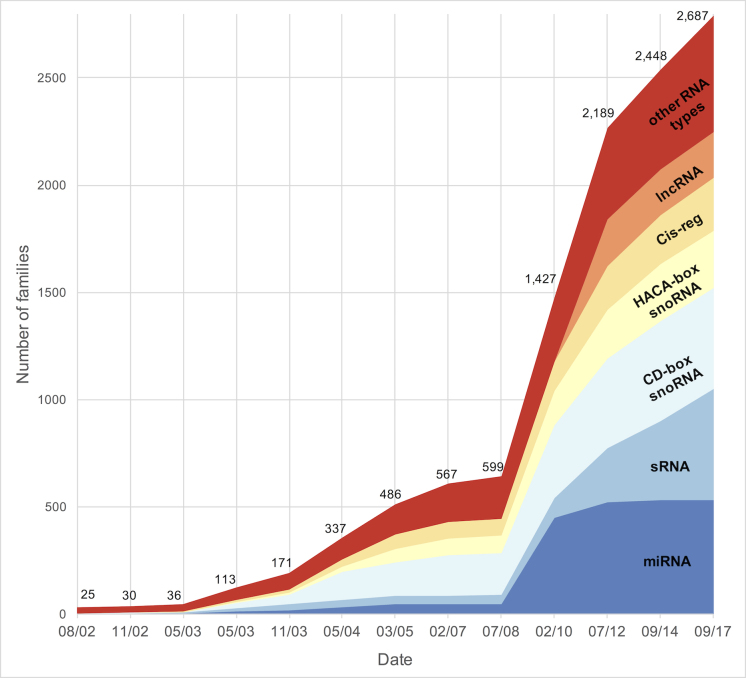
\includegraphics[height=7in]{figs/kalvari-17-fig1}
\end{center}
\vfill
\tiny \flushleft{Kalvari et al., 2018}
\end{slide}
%%%%%%%%%%%%%%%%%%%%%%%%%%%%%%%%%%%%%%%%%%%%%%%%%%%%%%%%%%%%%%%%%%%%
\begin{slide}
\begin{center}
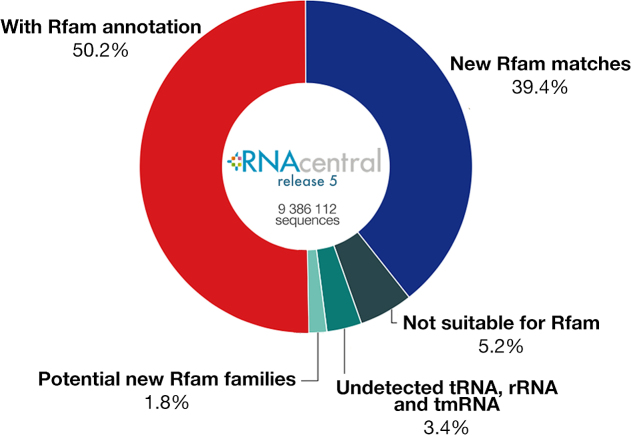
\includegraphics[height=7in]{figs/kalvari-2017-fig7}
\end{center}
\vfill
\tiny \flushleft{Kalvari et al., 2018}
\end{slide}
%%%%%%%%%%%%%%%%%%%%%%%%%%%%%%%%%%%%%%%%%%%%%%%%%%%%%%%%%%%%%%%%%%%%
%%%%%%%%%%%%%%%%%%%%%%%%%%%%%%%%%%%%%%%%%%%%%%%%%%%%%%%%%%%%%%%%%%%%%%
\begin{slide}
\begin{center}
  \textbf{Rfamseq: switch from subset of ENA to genome-centric database}
  \begin{itemize}  
  \item about 8000 reference genomes
  \item reduces redundancy
  \item more scalable
  \end{itemize}
\vspace{0.5in}
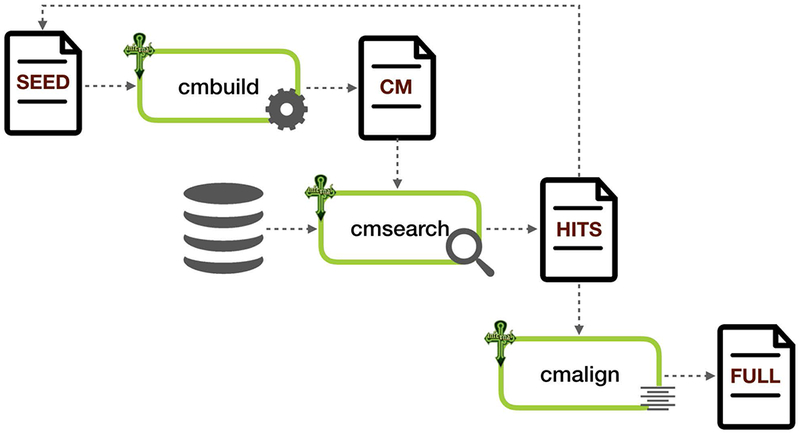
\includegraphics[height=4in]{figs/kalvari18-rfam-schema}
\end{center}    
\vfill
\tiny \flushleft{Kalvari et al., 2018}
\end{slide}
%%%%%%%%%%%%%%%%%%%%%%%%%%%%%%%%%%%%%%%%%%%%%%%%%%%%%%%%%%%%%%%%%%%%%%
\begin{slide}
\begin{center}
  \textbf{Rfamseq: switch from subset of ENA to genome-centric database}
  \begin{itemize}  
  \item about 8000 reference genomes
  \item reduces redundancy
  \item more scalable
  \end{itemize}

  \textbf{Rfamseq: genome-centric database means less flexible SEEDs}
  \begin{itemize}  
  \item previous requirement: SEED sequences must be in Rfamseq
  \item new approach allows any GenBank or RNAcentral sequence
  \item verification of sequences utilizes GenBank and RNAcentral API
  \end{itemize}
\end{center}    
\vfill
\end{slide}
%%%%%%%%%%%%%%%%%%%%%%%%%%%%%%%%%%%%%%%%%%%%%%%%%%%%%%%%%%%%%%%%%%%%%%
\begin{slide}
\begin{center}
  \textbf{Future directions for Rfam}
  \begin{itemize}  
  \item improve Rfam families based on crystal structures
  \item synchronize with mirBase
  \item use model reference coordinates to annotate important features 
  \item continue to add families
  \end{itemize}
\end{center}    
\vfill
\end{slide}
%%%%%%%%%%%%%%%%%%%%%%%%%%%%%%%%%%%%%%%%%%%%%%%%%%%%%%%%%%%%%%%%%%%%%%


\end{document}
%%%%%%%%%%%%%%%%%%%%%%%%%%%%%%%%%%%%%%%%%%%%%%%%%%%%%%%%%%%%%%%%%%%%
\begin{slide}

\begin{center}
\large{\textbf{Rfam is 16 years old}}
\end{center}

\bigskip

\scriptsize

%ref: ftp://ftp.sanger.ac.uk/pub/databases/Rfam/CURRENT/README
%ref: http://infernal.janelia.org
\begin{center}
\begin{tabular}{ccrrcc} \hline
     &         &    \# of & Infernal& Rfam & Infernal \\
year & release & families & version & head & team \\ \hline
2002 & 0.1     &        4 &     0.3 & SGJ  & SE  \\
2002 & 0.2     &       12 &     0.3 & SGJ  & SE  \\
2002 & 0.3     &       21 &     0.3 & SGJ  & SE  \\
2002 & 1.0     &       25 &     0.4 & SGJ  & SE  \\
2002 & 2.0     &       30 &     0.55 & SGJ  & SE  \\
2003 & 3.0     &       36 &     0.55 & SGJ  & SE  \\
2003 & 4.0     &      114 &     0.55 & SGJ  & SE  \\
2003 & 4.1     &      165 &     0.55 & SGJ  & SE  \\
2003 & 5.0     &      176 &     0.55 & SGJ  & SE  \\
2004 & 6.0     &      350 &     0.55 & SGJ  & SE  \\
2004 & 6.1     &      379 &     0.55& SGJ  & SE  \\
2005 & 7.0     &      503 &     0.55& SGJ  & SE  \\
%2004 & \multicolumn{5}{c}{My (EPN's) doctoral work on \sft{infernal} begins} \\
2007 & 8.0     &      574 &     0.7 & PG  & EN, DK, SE  \\
2007 & 8.1     &      607 &     0.81& PG  & EN, DK, SE  \\
2008 & 9.0     &      603 &     0.81& PG  & EN, DK, SE  \\
2008 & 9.1     &     1372 &     0.81& PG  & EN, DK, SE  \\
2010 & 10.0    &     1446 &     1.0  & PG  & EN, SE \\
2011 & 10.1    &     1973 &    1.0.2 & PG  & EN, SE \\
2012 & 11.0    &     2208 &   1.0.2 & SB, EN  & EN, SE \\
2014 & 12.0    &     2450 &   1.1.1 & SB, EN  & EN, SE \\
2016 & 12.1    &     2473 &   1.1.1 & AP  & EN, SE \\
2017 & 12.2    &     2588 &   1.1.2 & AP  & EN, SE \\
2017 & 12.3    &     2687 &   1.1.2 & AP  & EN, SE \\
2017 & 13.0    &     2686 &   1.1.2 & AP  & EN, SE \\
2018 & 14.0    &     2791 &   1.1.2 & AP  & EN, SE \\
2019 & 14.1    &     3016 &   1.1.2 & AP  & EN, SE \\
\end{tabular}

\end{center}

\tiny
SGJ: Sam Griffiths-Jones; SE: Sean Eddy; PG: Paul Gardner; EN: Eric
Nawrocki; DK: Diana Kolbe; \\ SB: Sarah Burge; AP: Anton Petrov
\normalsize


\vfill
\end{slide}
\begin{slide}
\begin{center}

\textbf{RNAcentral uses Rfam to annotate sequences}

\begin{itemize}
\item 16.5 million sequences
\item 50\% are from Rfam
\item 40\% have Rfam hits
\item  2\% are potential sources of new Rfam families
\end{itemize}

\end{center}
\vfill
\end{slide}
